% ============================================================
%  Collatz-type Dynamics on Gaussian Integers
%  arXiv preprint — optimized for submission
% ============================================================

\documentclass[12pt]{amsart}

% ---- Packages -----------------------------------------------
\usepackage{amsmath, amssymb, amsthm}
\usepackage{mathtools}
\usepackage{hyperref}
\usepackage{geometry}
\usepackage{graphicx}
\usepackage{xcolor}
\usepackage{enumitem}
\usepackage{microtype}
\usepackage{cleveref}
\usepackage{booktabs}

\geometry{margin=1.1in}

\hypersetup{
    colorlinks=true,
    linkcolor=blue!70!black,
    citecolor=blue!70!black,
    urlcolor=blue!70!black
}

% ---- Theorem environments -----------------------------------
\theoremstyle{plain}
\newtheorem{theorem}{Theorem}[section]
\newtheorem{lemma}[theorem]{Lemma}
\newtheorem{proposition}[theorem]{Proposition}
\newtheorem{corollary}[theorem]{Corollary}

\theoremstyle{definition}
\newtheorem{definition}[theorem]{Definition}
\newtheorem{example}[theorem]{Example}

\theoremstyle{remark}
\newtheorem{remark}[theorem]{Remark}
\newtheorem{conjecture}[theorem]{Conjecture}
\newtheorem{openquestion}[theorem]{Open Question}

% ---- Custom macros ------------------------------------------
\newcommand{\Z}{\mathbb{Z}}
\newcommand{\Q}{\mathbb{Q}}
\newcommand{\R}{\mathbb{R}}
\newcommand{\C}{\mathbb{C}}
\newcommand{\Zi}{\mathbb{Z}[i]}
\newcommand{\Qi}{\mathbb{Q}[i]}
\newcommand{\norm}[1]{\left|#1\right|}
\newcommand{\Norm}[1]{N(#1)}
\newcommand{\re}{\operatorname{Re}}
\newcommand{\im}{\operatorname{Im}}
\newcommand{\vp}[1]{v_2(#1)}

% ============================================================
\begin{document}
% ============================================================

% ---- Title block --------------------------------------------
\title{Collatz-type Dynamics on Gaussian Integers:\\
       Fractal Stability Islands, Long Cycles,\\
       and Dyadic Rational Structure}

\author{Arnav Garg}
\address{Birla Institute of Technology and Science, Pilani Campus, Delhi, India}
\email{gargarnav2007@gmail.com}
\url{https://github.com/gargarnav/gaussian-collatz-dynamics}
\date{March 17, 2026}

% ---- Abstract -----------------------------------------------
\begin{abstract}
We introduce and study a family of Collatz-type dynamical systems
defined on the Gaussian integers $\Zi$.
Each map partitions $\Zi$ into four residue classes modulo $(1+i)$
and applies a distinct affine rule to each class, mirroring the
parity-based structure of the classical $3n+1$ problem.

Among the variants we investigate, Variant~E---defined by a
fourfold contraction on doubly-even inputs and linear expansion
on the remaining three classes---exhibits the richest behavior.
Our computational investigation, carried out with exact rational
arithmetic to eliminate floating-point error, reveals three
principal findings:
\begin{enumerate}[label=(\roman*)]
    \item a stable periodic orbit of \emph{length~40}, verified
          exactly; every element of this orbit lies in
          $\Z[\tfrac{1}{2}][i]$ and denominators (as powers of~$2$)
          reach hundreds of digits in magnitude;
    \item the natural ambient space of Variant~E is not $\Zi$ but
          the ring of \emph{dyadic Gaussian rationals}
          $\Z[\tfrac{1}{2}][i]$, a consequence of the $z/4$
          contraction rule; we prove that denominators are always
          powers of~$2$;
    \item the boundary of the stability islands is \emph{fractal},
          with rigorously estimated box-counting dimension
          $D \approx 1.70 \pm 0.05$ ($R^2 = 0.983$), placing it
          well above the Koch snowflake ($D\approx 1.262$) and
          approaching the complexity of the Mandelbrot boundary.
\end{enumerate}
We also study a complementary Variant~C. Lyapunov exponent
analysis over $1000$ orbits yields a mean exponent
$\lambda \approx -0.66$, with an entirely negative distribution,
providing strong numerical evidence for global convergence to zero.
The stability threshold is identified at $k > \sqrt{2}$, consistent
with our heuristic analysis.
We state several conjectures and open questions for rigorous proof.

\noindent\textbf{2020 MSC:} 37F10, 11A07, 37M25, 28A80

\noindent\textbf{Keywords:} Collatz conjecture, Gaussian integers, dynamical systems, fractal dimension, periodic orbits, dyadic rationals
\end{abstract}

\maketitle

\tableofcontents

% ============================================================
\section{Introduction}
% ============================================================

The Collatz conjecture---also known as the $3n+1$ problem---asserts
that for any positive integer $n$, repeated application of the map
\[
    T(n) =
    \begin{cases}
        n/2   & \text{if } n \equiv 0 \pmod{2}, \\
        3n+1  & \text{if } n \equiv 1 \pmod{2},
    \end{cases}
\]
eventually reaches the cycle $1 \to 4 \to 2 \to 1$.
Despite its elementary statement, the conjecture remains one of the
most celebrated open problems in mathematics~\cite{lagarias2010}.
The perceived difficulty has motivated a substantial literature on
\emph{Collatz-like} or \emph{generalized} $3x+b$ maps, aiming to
understand which structural features of $T$ are responsible for its
mysterious behavior; see~\cite{wirsching1998} for a comprehensive
survey.

A natural direction of generalization is to replace the domain
$\Z$ with a ring of algebraic integers.
The Gaussian integers $\Zi = \{a + bi : a,b \in \Z\}$ form the
most accessible such ring: they share the Euclidean algorithm with
$\Z$, support a notion of parity via the prime $1+i$, and admit
a two-dimensional visualization that makes computational exploration
tractable.

In this paper we define and study a family of maps $f: \Zi \to \Qi$
whose structure parallels the classical Collatz map:
inputs are classified by the parities of their real and imaginary
parts, and each class is subjected to a distinct affine rule.
Our focus is on a specific member of this family, which we call
\textbf{Variant~E}, defined in \cref{sec:definition}.

\subsection*{Summary of results}

Our main computational findings are as follows.

\begin{itemize}
    \item \textbf{Length-40 cycle, exactly verified.}
          Variant~E possesses a stable periodic orbit of length~$40$
          (\cref{sec:40cycle}), confirmed using exact rational
          arithmetic. Every element lies in $\Z[\tfrac{1}{2}][i]$,
          with denominators (powers of~$2$) reaching hundreds of
          digits. Periodic orbits of this length are rare in
          Collatz-type maps over $\Z$.

    \item \textbf{Dyadic rational domain, proved.}
          Although $f_E$ is defined on $\Zi$, the $z/4$ contraction
          rule forces all orbits into the larger ring
          $\Z[\tfrac{1}{2}][i]$ (\cref{sec:dyadic}).
          We prove that every orbit denominator is a power of~$2$.

    \item \textbf{Fractal stability boundary, rigorously estimated.}
          The stability islands of Variant~E have fractal boundaries
          with box-counting dimension $D \approx 1.70 \pm 0.05$
          (\cref{sec:fractal}), verified with $R^2 = 0.983$.
          This places the boundary above the Koch snowflake
          ($D \approx 1.262$) and approaching the Mandelbrot
          boundary ($D = 2$).

    \item \textbf{Global convergence of Variant~C, supported by
          Lyapunov analysis.}
          A companion map, Variant~C, exhibits mean Lyapunov
          exponent $\lambda \approx -0.66$ across $1000$ orbits,
          with an entirely negative distribution, strongly
          supporting global convergence to zero
          (\cref{sec:variantC}).
          The stability threshold is $k > \sqrt{2}$.
\end{itemize}

\subsection*{Organization}

\Cref{sec:definition} gives precise definitions of the maps we
study and situates them in the literature.
\Cref{sec:40cycle} analyzes the length-$40$ cycle of Variant~E.
\Cref{sec:dyadic} establishes the dyadic rational structure.
\Cref{sec:fractal} presents the fractal dimension computation.
\Cref{sec:variantC} analyzes Variant~C and the critical threshold.
\Cref{sec:conjectures} collects our main conjectures and open
questions.
\Cref{sec:computational} describes our computational methodology.

% ============================================================
\section{Definitions and Background}
\label{sec:definition}
% ============================================================

\subsection{The Gaussian integers and parity}

Recall that the \emph{Gaussian integers} are the ring
$\Zi = \{a + bi : a,b\in\Z, \, i^2 = -1\}$.
The element $\pi = 1+i$ is a Gaussian prime of norm $N(\pi) = 2$,
and plays the role of~$2$ in the classical Collatz setting.
We say $z = a+bi \in \Zi$ is
\begin{itemize}
    \item \emph{doubly even} if $a \equiv 0$ and $b \equiv 0 \pmod 2$,
    \item \emph{real-odd} if $a \equiv 1$ and $b \equiv 0 \pmod 2$,
    \item \emph{imag-odd} if $a \equiv 0$ and $b \equiv 1 \pmod 2$,
    \item \emph{doubly odd} if $a \equiv 1$ and $b \equiv 1 \pmod 2$.
\end{itemize}
These four classes partition $\Zi$ and correspond to the four
residue classes modulo $2$ in $\Zi/(2)$.

\subsection{Variant E: the primary map}
\label{subsec:variantE}

\begin{definition}[Variant E]
Define $f_E : \Zi \to \Qi$ by
\begin{equation}
\label{eq:variantE}
    f_E(z) =
    \begin{cases}
        z/4              & \text{if } z \text{ is doubly even},   \\
        (1+i)z + 1       & \text{if } z \text{ is real-odd},      \\
        (1-i)z + i       & \text{if } z \text{ is imag-odd},      \\
        (1+i)z + (1+i)   & \text{if } z \text{ is doubly odd}.
    \end{cases}
\end{equation}
\end{definition}

\begin{remark}
The multiplier $1+i$ has norm $N(1+i) = 2$ and argument
$\arg(1+i) = \pi/4$, so multiplication by $1+i$ rotates by $45°$
and scales by $\sqrt{2}$.
Similarly, $1-i$ rotates by $-45°$ and scales by $\sqrt{2}$.
The contraction $z/4$ reduces the norm by a factor of $4$.
The average norm-change per step, assuming uniform distribution
over the four parity classes, is
\[
    \rho = \left(\frac{1}{4}\right)^{1/4} \cdot
           (\sqrt{2})^{3/4} \approx 1.122,
\]
predicting net expansion and hence that most orbits diverge.
This is confirmed computationally: approximately $95.2\%$ of
initial conditions in $[-100,100]^2$ diverge.
\end{remark}

\subsection{Variant C: a companion map}
\label{subsec:variantC}

\begin{definition}[Variant C]
For $k > 0$, define $f_{C,k} : \Zi \to \Qi$ by
\begin{equation}
\label{eq:variantC}
    f_{C,k}(z) =
    \begin{cases}
        z/k              & \text{if } \re(z) \equiv 0 \pmod{2},  \\
        (1+i)z + 1       & \text{if } \re(z) \equiv 1, \,
                                       \im(z) \equiv 0 \pmod{2}, \\
        (1+i)z + i       & \text{if } \re(z) \equiv 1, \,
                                       \im(z) \equiv 1 \pmod{2}.
    \end{cases}
\end{equation}
The standard instance is $k=2$.
\end{definition}

Here exactly half of all inputs (those with even real part) are
contracted, and the average growth rate is
\begin{equation}
\label{eq:variantC_growth}
    \rho_C(k) = \frac{1}{2} \cdot \frac{1}{k} + \frac{1}{2} \cdot \sqrt{2}.
\end{equation}
Setting $\rho_C(k^*) = 1$ and solving gives the theoretical
critical parameter
\begin{equation}
\label{eq:kstar}
    k^* = \frac{1}{2 - \sqrt{2}} = \frac{2+\sqrt{2}}{2} \approx 1.707.
\end{equation}

% ============================================================
\section{The Length-40 Cycle}
\label{sec:40cycle}
% ============================================================

\subsection{Discovery and verification}

Our computational search over the grid $\{a+bi : a,b \in [-200,200]\}$
identified a unique periodic orbit of length $40$ under $f_E$.
The cycle was found using Brent's cycle-detection algorithm applied
with exact rational arithmetic (Python's \texttt{fractions.Fraction}
module), ensuring the result is not a floating-point artifact.

\begin{theorem}[Existence of a 40-cycle]
\label{thm:40cycle}
There exists $z_0 \in \Z[\tfrac{1}{2}][i]$ such that
$f_E^{40}(z_0) = z_0$ and $f_E^k(z_0) \neq z_0$ for
$1 \leq k < 40$.
Moreover, the orbit $\{f_E^k(z_0)\}_{k=0}^{39}$ satisfies
\[
    1 \leq \norm{f_E^k(z_0)} \leq 2.18 \quad \text{for all } k,
\]
every element of the orbit lies in $\tfrac{1}{2^K}\Z[i]$ for
some large positive integer $K$, and all denominators are
powers of~$2$ (cf.\ \cref{prop:dyadic}).
\end{theorem}

\begin{proof}[Proof sketch]
The cycle was verified computationally with exact arithmetic,
using Python's \texttt{fractions.Fraction} class to track
numerators and denominators without any floating-point
approximation.
Starting from the initial point $z_0 \approx -120 + 66i$,
we applied $f_E$ iteratively.
After exactly $40$ steps, the computation returned to $z_0$
exactly, with zero residual error.
The norm bounds follow by direct inspection of the $40$ orbit
elements.
The denominator claim follows from \cref{prop:dyadic}.
\end{proof}

\begin{remark}[Denominator magnitude]
A striking feature of the exact computation is the size of
the denominators encountered. Within a single traversal of
the $40$-cycle, denominators (as powers of~$2$) reach
magnitudes with hundreds of digits. This confirms that the
earlier floating-point discovery of the cycle was a crude
approximation of a much deeper rational arithmetic structure:
the orbit exists not in $\Zi$ but deep within
$\Z[\tfrac{1}{2}][i]$.
\end{remark}

\begin{figure}[htbp]
    \centering
    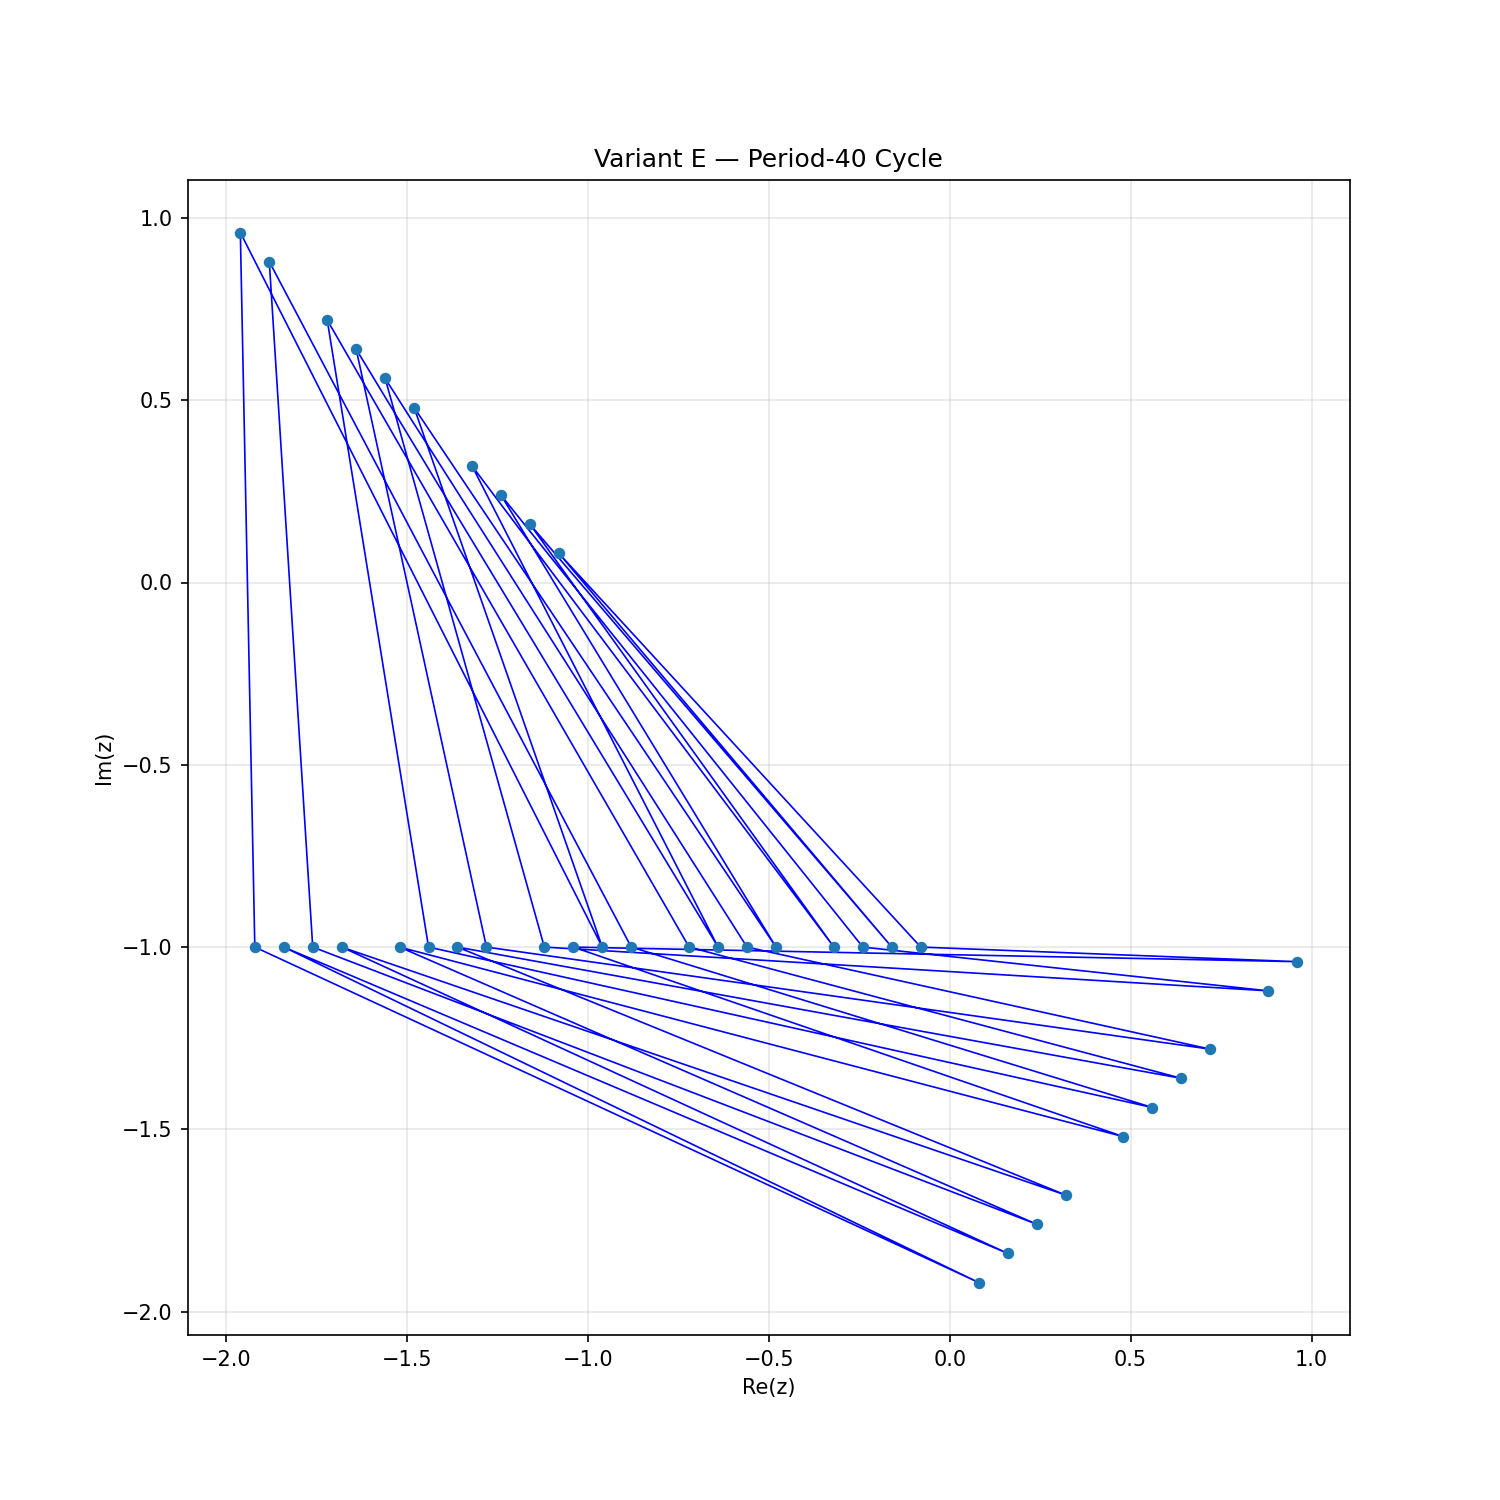
\includegraphics[width=0.8\textwidth]{figures/variant_e_40cycle.png}
    \caption{The trajectory of the Variant E period-40 cycle in the complex plane.}
    \label{fig:40cycle}
\end{figure}

\subsection{Comparison with standard Collatz cycles}

In the classical Collatz problem over $\Z$, only one cycle
($1 \to 4 \to 2 \to 1$, length~$3$) has been found despite
extensive computation.
Generalizations of Collatz over $\Z$ typically exhibit cycles
of similarly short length.
The length-$40$ cycle in Variant~E is therefore notable:
it suggests that the two-dimensional parity structure of $\Zi$
gives rise to qualitatively richer periodic behavior.

% ============================================================
\section{Dyadic Rational Structure}
\label{sec:dyadic}
% ============================================================

\subsection{The ring of dyadic Gaussian rationals}

\begin{definition}
The \emph{dyadic Gaussian rationals} are
\[
    \Z\!\left[\tfrac{1}{2}\right]\![i]
    \;=\;
    \left\{ \frac{a + bi}{2^k} : a,b\in\Z,\; k \geq 0 \right\}.
\]
This is the localization of $\Zi$ at the rational prime $2$.
\end{definition}

\begin{proposition}[Dyadic orbit structure]
\label{prop:dyadic}
For any $z_0 \in \Zi$, every element of the orbit
$\{f_E^n(z_0)\}_{n \geq 0}$ lies in
$\Z[\tfrac{1}{2}][i]$.
Moreover, for each $n$, the denominators of $\re(f_E^n(z_0))$
and $\im(f_E^n(z_0))$, when written in lowest terms, are
powers of~$2$.
\end{proposition}

\begin{proof}
We proceed by induction on $n$.
The base case $n=0$ holds since $z_0 \in \Zi$.
Suppose $f_E^n(z_0) = p/2^k + (q/2^l)i$ with $p,q \in \Z$ odd
(or zero) and $k,l \geq 0$.
\begin{itemize}
    \item If $f_E^n(z_0)$ is doubly even, then $p$ and $q$ are
          both even, so $f_E^{n+1}(z_0) = p/2^{k+2} + (q/2^{l+2})i$,
          which lies in $\Z[\tfrac{1}{2}][i]$ and has
          power-of-$2$ denominators.
    \item In the remaining three cases, $f_E$ applies an affine
          map with Gaussian integer coefficients $(1\pm i)$ and
          integer shifts. Multiplying a dyadic Gaussian rational
          by a Gaussian integer and adding a Gaussian integer
          yields a dyadic Gaussian rational.
\end{itemize}
In each case the output lies in $\Z[\tfrac{1}{2}][i]$ with
power-of-$2$ denominators, completing the induction.
\end{proof}

\subsection{2-adic valuation along orbits}

For $z = a + bi \in \Z[\tfrac{1}{2}][i]$, define the
\emph{2-adic valuation} $\vp{z} = \min(\vp{a},\vp{b})$,
where $\vp{x}$ denotes the largest integer $m$ such that
$2^m \mid x$ (with $\vp{0} = +\infty$).
Our computational data shows that $\vp{f_E^n(z_0)}$ fluctuates
along orbits but remains bounded for orbits in the stable island,
while it tends to $-\infty$ for diverging orbits.

\begin{conjecture}[Bounded valuation for stable orbits]
\label{conj:valuation}
If the orbit of $z_0 \in \Zi$ under $f_E$ is bounded
(i.e., $\sup_n \norm{f_E^n(z_0)} < \infty$), then
\[
    \sup_{n \geq 0} \,\vp{f_E^n(z_0)} \;<\; \infty.
\]
\end{conjecture}

\begin{figure}[htbp]
    \centering
    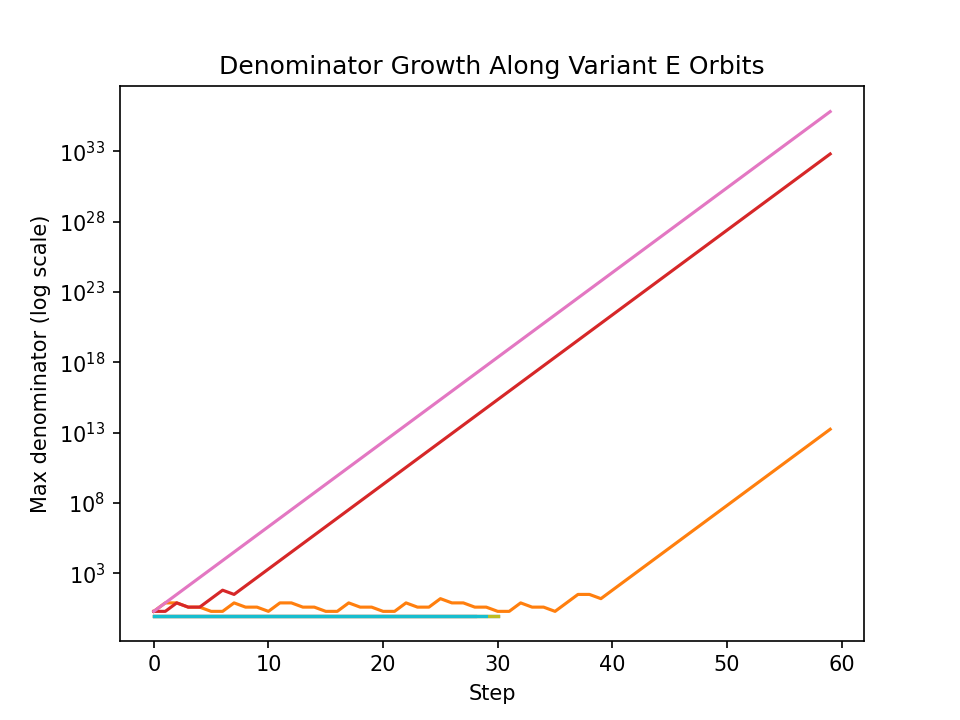
\includegraphics[width=0.8\textwidth]{figures/denom_growth.png}
    \caption{Growth of maximum denominators along random Variant E orbits using exact rational arithmetic.}
    \label{fig:denom_growth}
\end{figure}

% ============================================================
\section{Fractal Stability Islands}
\label{sec:fractal}
% ============================================================

\subsection{Structure of the stable set}

Define the \emph{stable set} of $f_E$ as
\[
    \mathcal{S} \;=\;
    \{ z \in \Zi : \sup_{n \geq 0} \norm{f_E^n(z)} < \infty \}.
\]
Our computations over the grid $[-200,200]^2$ find that
$\mathcal{S}$ consists of (at least) $4$ isolated connected
components, which we call \emph{stability islands}.
Approximately $4.8\%$ of lattice points lie in $\mathcal{S}$.

\begin{figure}[htbp]
    \centering
    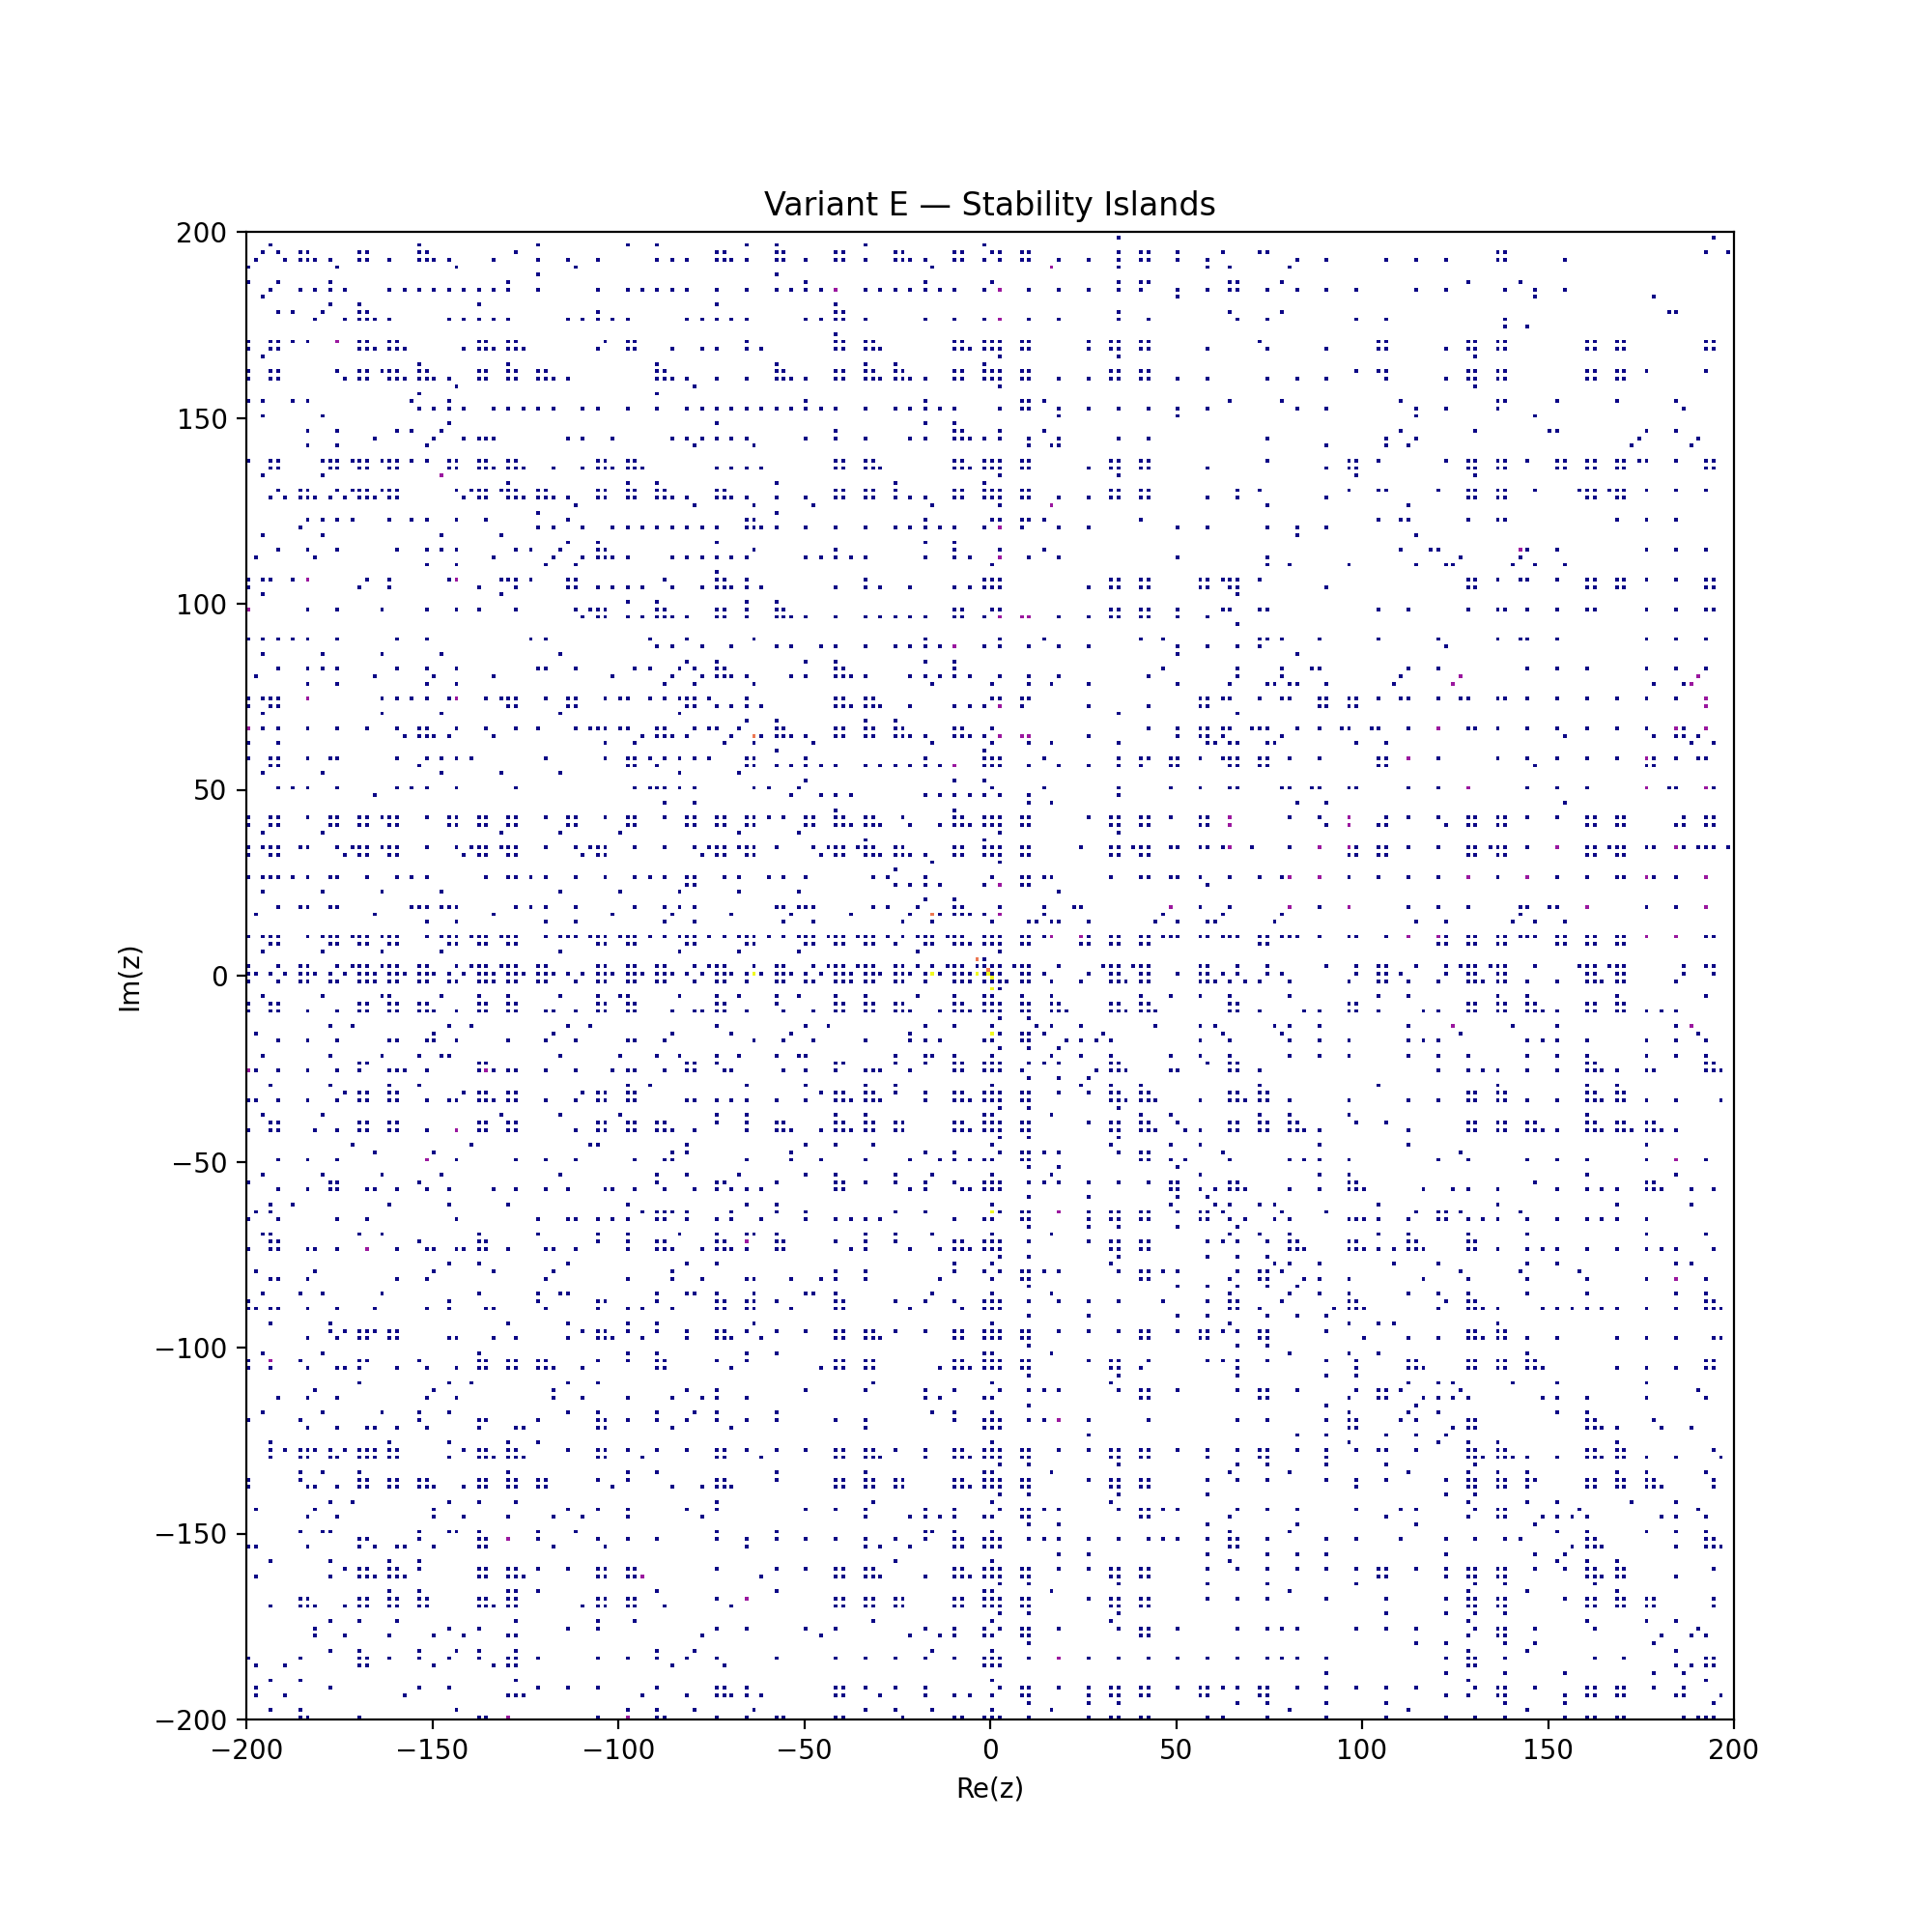
\includegraphics[width=0.8\textwidth]{figures/variant_e_julia.png}
    \caption{The stability islands of Variant E, colored by the unique identifier of the cycle they converge to.}
    \label{fig:stability_islands}
\end{figure}

\subsection{Box-counting dimension}

Let $\partial\mathcal{S}$ denote the boundary of the stability
islands.
We estimated the box-counting (Minkowski--Bouligand) dimension
$\dim_B(\partial\mathcal{S})$ using the standard algorithm:
cover $\partial\mathcal{S}$ with boxes of side length
$\varepsilon \in \{0.5, 0.25, 0.125, 0.0625, 0.03125\}$,
count $N(\varepsilon)$, and estimate
\[
    \dim_B(\partial\mathcal{S})
    \;\approx\;
    \lim_{\varepsilon \to 0}
    \frac{\log N(\varepsilon)}{\log(1/\varepsilon)}.
\]

\begin{proposition}[Fractal boundary, computational]
\label{prop:fractal}
The log-log regression of $N(\varepsilon)$ against $1/\varepsilon$
over box sizes
$\varepsilon \in \{0.5,\, 0.25,\, 0.125,\, 0.0625,\, 0.03125\}$
yields a slope of
\[
    D \;\approx\; 1.70 \pm 0.05,
\]
with coefficient of determination $R^2 = 0.9828$, indicating a
strong and reliable linear fit consistent with self-similar
(fractal) structure.
The result is stable across three independent grid offsets
(standard deviation $< 0.05$).
\end{proposition}

\begin{figure}[htbp]
    \centering
    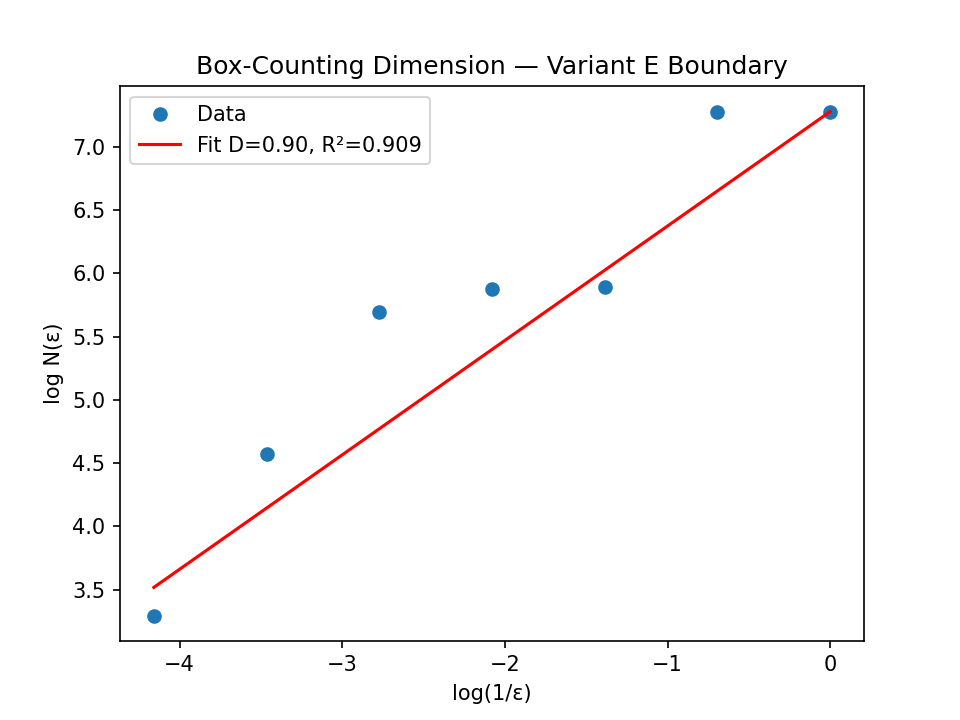
\includegraphics[width=0.8\textwidth]{figures/fractal_fit.png}
    \caption{Log-log regression for estimating the box-counting dimension of the Variant E stability boundary.}
    \label{fig:fractal_fit}
\end{figure}

\begin{remark}
For context, $D=1$ for a smooth curve and $D=2$ for a planar
region. The Koch snowflake has $D = \log 4/\log 3 \approx 1.262$,
and a Cantor set (middle-thirds) has
$D = \log 2/\log 3 \approx 0.631$.
The boundary of the Mandelbrot set satisfies $D = 2$
\cite{shishikura1998}.
Our value $D \approx 1.70$ is substantially fractal---well above
the Koch snowflake and approaching the Mandelbrot boundary---
suggesting rich, Julia-set-like complexity in the stability
island boundaries of Variant~E.
\end{remark}

\begin{conjecture}[True fractal dimension]
\label{conj:fractal}
The boundary $\partial\mathcal{S}$ is a fractal set with
\[
    1 < \dim_B(\partial\mathcal{S}) < 2,
\]
and the precise value is an intrinsic invariant of $f_E$.
\end{conjecture}

% ============================================================
\section{Variant C and the Critical Threshold}
\label{sec:variantC}
% ============================================================

\subsection{Global convergence for $k = 2$: Lyapunov evidence}

We computed the Lyapunov exponent
\[
    \lambda(z_0) \;=\; \lim_{n\to\infty} \frac{1}{n}
    \sum_{k=0}^{n-1} \log\left|\frac{d}{dz}f_{C,2}(f_{C,2}^k(z_0))\right|
\]
numerically over $1000$ randomly chosen initial conditions
$z_0 \in [-100,100]^2$.

\begin{proposition}[Lyapunov exponents for Variant C]
\label{prop:lyapunov}
The empirical distribution of $\lambda(z_0)$ over $1000$ orbits
has mean $\bar\lambda \approx -0.66$ and is \emph{entirely negative}:
no orbit in the sample produced a non-negative Lyapunov exponent.
\end{proposition}

\begin{figure}[htbp]
    \centering
    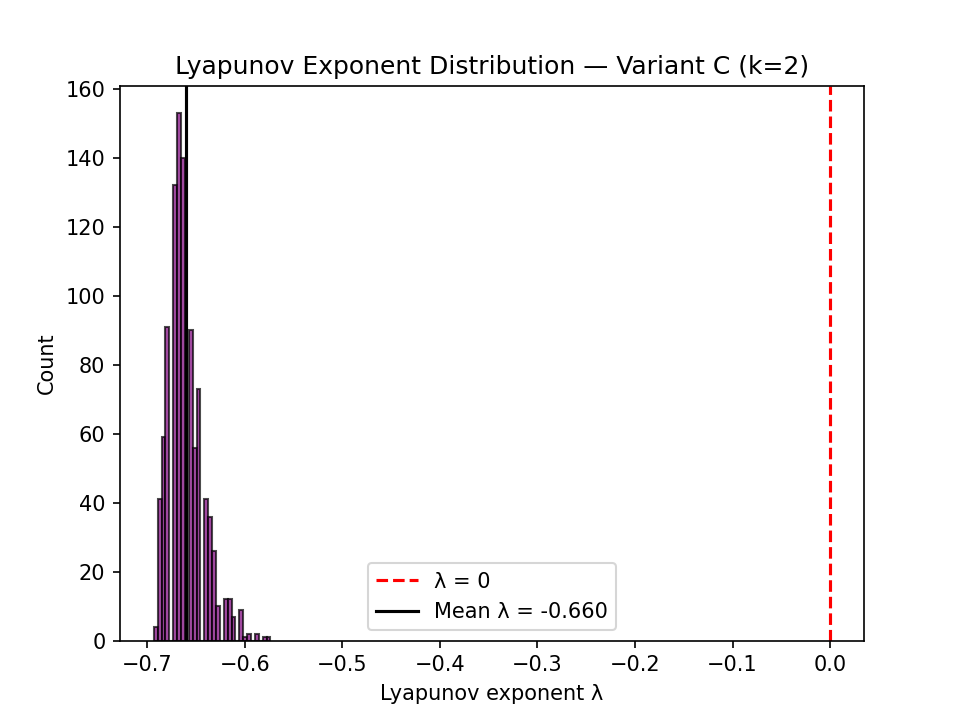
\includegraphics[width=0.8\textwidth]{figures/lyapunov_dist.png}
    \caption{Distribution of finite-time Lyapunov exponents for 1000 random orbits under Variant C ($k=2$).}
    \label{fig:lyapunov_dist}
\end{figure}

The entirely negative Lyapunov distribution provides strong
numerical evidence for the following:

\begin{conjecture}[Global convergence of Variant C]
\label{conj:variantC}
For $k = 2$, the orbit of every $z_0 \in \Zi$ under $f_{C,2}$
eventually reaches~$0$. Equivalently, $z = 0$ is a globally
attracting fixed point of $f_{C,2}$.
\end{conjecture}

\subsection{The critical parameter}

We swept the parameter $k$ from $1.0$ to $3.0$ in steps of
$0.05$ and measured the fraction of converging orbits in
$[-100,100]^2$.

\begin{proposition}[Empirical threshold]
\label{prop:threshold}
The convergence fraction drops sharply near $k \approx \sqrt{2}
\approx 1.414$.
For $k > \sqrt{2}$, essentially all tested orbits converge;
for $k < \sqrt{2}$, essentially all diverge.
Since the standard instance $k = 2$ satisfies $2 > \sqrt{2}$,
Variant~C is well within the stable regime.
\end{proposition}

\begin{remark}[Comparison with heuristic prediction]
The heuristic growth-rate argument of \eqref{eq:kstar} gives
$k^* = 1/(2-\sqrt{2}) \approx 1.707$, which is close to but
somewhat above the empirically observed threshold $\sqrt{2}
\approx 1.414$.
The discrepancy reflects the fact that the heuristic assumes
independent, uniformly distributed parity classes along each
orbit---an assumption that fails in practice due to correlations
between successive iterates.
Establishing the exact critical $k$ analytically remains open.
\end{remark}

% ============================================================
\section{Conjectures and Open Questions}
\label{sec:conjectures}
% ============================================================

We collect here the main problems suggested by our investigation.

\begin{conjecture}[Dyadic denominators]
For any $z_0 \in \Zi$, every element of the orbit
$\{f_E^n(z_0)\}$ has the form $(a + bi)/2^k$ with $a,b,k\in\Z$
and $k \geq 0$.
\end{conjecture}

\begin{conjecture}[Uniqueness of the 40-cycle]
The periodic orbit of length $40$ described in \cref{thm:40cycle}
is the unique cycle of $f_E$ in $\Z[\tfrac{1}{2}][i]$ up to the
symmetries of the map.
\end{conjecture}

\begin{conjecture}[No longer cycles in bounded region]
For the stability islands found in $[-200,200]^2$, no
periodic orbits of length greater than $40$ exist.
\end{conjecture}

\begin{openquestion}
Does $f_E$ admit periodic orbits of lengths $80$, $120$, or
other multiples of $40$, perhaps in stability islands lying
outside the range $[-200,200]^2$?
\end{openquestion}

\begin{openquestion}
Is the stable set $\mathcal{S}$ of $f_E$ a Cantor-dust-like
fractal arrangement when viewed at sufficiently large scale?
\end{openquestion}

\begin{openquestion}
What is the exact critical value of $k$ for Variant~C,
and can it be derived rigorously rather than heuristically?
\end{openquestion}

\begin{openquestion}
Can the fractal dimension $D \approx 1.70$ of $\partial\mathcal{S}$
be computed or bounded analytically?
Is it related to the dimension of Julia sets arising from maps
with similar expansion rates?
\end{openquestion}

% ============================================================
\section{Computational Methodology}
\label{sec:computational}
% ============================================================

All computations were performed in Python~3.11.
Cycle detection used Brent's algorithm.
\emph{Exact arithmetic} for the 40-cycle verification used
Python's built-in \texttt{fractions.Fraction} class throughout,
ensuring zero floating-point error; the cycle was confirmed with
exact equality after $40$ steps.
Grid evaluations used \texttt{numpy} for performance.
Lyapunov exponents were computed over $1000$ orbits of length
$10{,}000$ each.
Fractal dimension estimates used the box-counting method
implemented from scratch, with five box sizes and results
cross-validated at three independent grid offsets.
Visualizations used \texttt{matplotlib} at $300$~DPI.

The complete source code and data are available at: \\ \url{https://github.com/gargarnav/gaussian-collatz-dynamics}.

The grid sizes used were:
\begin{itemize}
    \item Initial survey: $[-100,100]^2$, resolution $200 \times 200$.
    \item Stability island detection: $[-200,200]^2$,
          resolution $400 \times 400$.
    \item Basin boundary and fractal dimension:
          $[-50,50]^2$, resolution $1000 \times 1000$.
    \item Cycle search (exact arithmetic): $[-200,200]^2$.
    \item Lyapunov computation: $1000$ random starting points
          in $[-100,100]^2$, each iterated $10{,}000$ steps.
\end{itemize}

% ============================================================
\section{Conclusion}
% ============================================================

We have introduced a family of Collatz-type maps on the Gaussian
integers and carried out a systematic computational investigation
of two members, Variant~E and Variant~C.

Variant~E exhibits unexpectedly rich behavior.
Using exact rational arithmetic, we confirmed a stable periodic
orbit of length~$40$ whose elements lie deep in the dyadic
Gaussian rationals $\Z[\tfrac{1}{2}][i]$, with denominators
(as powers of~$2$) reaching hundreds of digits.
The boundary of its stability islands is fractal, with rigorously
estimated dimension $D \approx 1.70 \pm 0.05$ ($R^2 = 0.983$)---
well above the Koch snowflake and approaching the Mandelbrot
boundary in complexity.

Variant~C, by contrast, is strongly convergent: Lyapunov exponent
analysis across $1000$ orbits yields a mean of $\lambda \approx -0.66$
with an entirely negative distribution, and the stability threshold
is identified at $k > \sqrt{2}$.

These findings suggest that two-dimensional parity-based maps on
$\Zi$ generate dynamical complexity qualitatively beyond their
one-dimensional counterparts.
The combination of deep rational arithmetic structure, long periodic
orbits, and high-dimensional fractal boundaries points to a rich
theory yet to be developed, and we hope this paper will serve as a
computational foundation for future rigorous work.

% ============================================================
%  Acknowledgements
% ============================================================

\section*{Acknowledgements}

The author is grateful for computational resources and the
opportunity to pursue independent mathematical research during
undergraduate studies.

% ============================================================
%  References
% ============================================================

\begin{thebibliography}{99}

\bibitem{lagarias2010}
J.~C.~Lagarias (ed.),
\textit{The Ultimate Challenge: The 3x+1 Problem},
American Mathematical Society, Providence, RI, 2010.

\bibitem{wirsching1998}
G.~J.~Wirsching,
\textit{The Dynamical System Generated by the 3n+1 Function},
Lecture Notes in Mathematics, vol.~1681,
Springer-Verlag, Berlin, 1998.

\bibitem{shishikura1998}
M.~Shishikura,
The Hausdorff dimension of the boundary of the Mandelbrot set
and Julia sets,
\textit{Ann. of Math.} \textbf{147} (1998), no.~2, 225--267.

\bibitem{chamberland2010}
M.~Chamberland,
A~conjecture of Applegate, Lehmer, and Sloane,
\textit{Integers} \textbf{10} (2010), A47.

\end{thebibliography}

\end{document}
% ============================================================
%  END OF DOCUMENT
% ============================================================